\documentclass{article}
\usepackage{amsmath}
\usepackage{enumerate}
\usepackage{listings}
\usepackage{moreverb}
\usepackage[margin=1in]{geometry}
\usepackage{graphicx}
\usepackage{dsfont}
\title{STA 360: Lab 6}
\author{Michael Lin}

\begin{document}
\maketitle

\begin{enumerate}
\item Since all means are 0, the full conditional for each of the three variables are derived as follows:
\begin{align*}
X|Y,Z &\sim N(\Sigma_{X,(Y,Z)}\Sigma_{Y,Z}^{-1}\begin{bmatrix}
Y \\
Z
\end{bmatrix}, \Sigma_X-\Sigma_{X,(Y,Z)}\Sigma_{Y,Z}^{-1}\Sigma_{(Y,Z),X}) \\
&= N(\begin{bmatrix} 0.9& 0.1 \end{bmatrix} {\begin{bmatrix} 1& 0.1 \\ 0.1& 1 \end{bmatrix}}^{-1} \begin{bmatrix}Y \\Z\end{bmatrix},
1-\begin{bmatrix}0.9& 0.1 \end{bmatrix}{\begin{bmatrix} 1& 0.1 \\ 0.1& 1 \end{bmatrix}}^{-1}\begin{bmatrix}0.9\\0.1\end{bmatrix}) \\
&= N(0.89899Y+0.01010Z, 0.18990) \\
Y|X,Z &\sim N(\Sigma_{Y,(X,Z)}\Sigma_{X,Z}^{-1}\begin{bmatrix}
X \\
Z
\end{bmatrix}, \Sigma_Y-\Sigma_{Y,(X,Z)}\Sigma_{X,Z}^{-1}\Sigma_{(X,Z),Y}) \\
&= N(\begin{bmatrix} 0.9& 0.1 \end{bmatrix} {\begin{bmatrix} 1& 0.1 \\ 0.1& 1 \end{bmatrix}}^{-1} \begin{bmatrix}X \\Z\end{bmatrix},
1-\begin{bmatrix}0.9& 0.1 \end{bmatrix}{\begin{bmatrix} 1& 0.1 \\ 0.1& 1 \end{bmatrix}}^{-1}\begin{bmatrix}0.9\\0.1\end{bmatrix}) \\
&= N(0.89899X+0.01010Z, 0.18990)\\
Z|X,Y &\sim N(\Sigma_{Z,(X,Y)}\Sigma_{X,Y}^{-1}\begin{bmatrix}
X \\
Y
\end{bmatrix}, \Sigma_Z-\Sigma_{Z,(X,Y)}\Sigma_{X,Y}^{-1}\Sigma_{(X,Y),Z}) \\
&= N(\begin{bmatrix} 0.1 & 0.1 \end{bmatrix} {\begin{bmatrix} 1 & 0.9 \\ 0.9& 1 \end{bmatrix}}^{-1} \begin{bmatrix}X \\Y\end{bmatrix},
1-\begin{bmatrix}0.1& 0.1 \end{bmatrix}{\begin{bmatrix} 1& 0.9 \\ 0.9& 1 \end{bmatrix}}^{-1}\begin{bmatrix}0.1\\0.1\end{bmatrix}) \\
&= N(0.052632X+0.052632Y, 0.98947)
\end{align*}


\item See R code. Below are the traceplot and autocorrelation function plot for X:

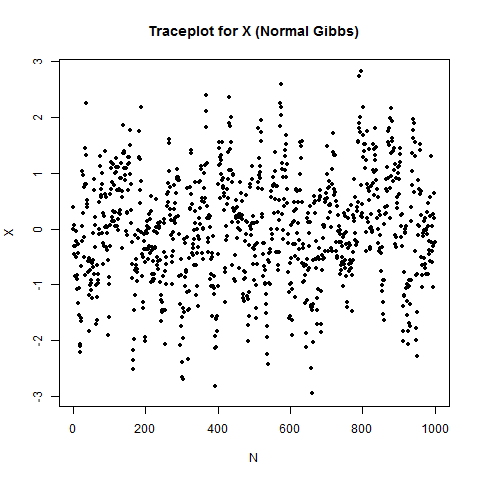
\includegraphics[scale=0.4]{tracenorm.png}
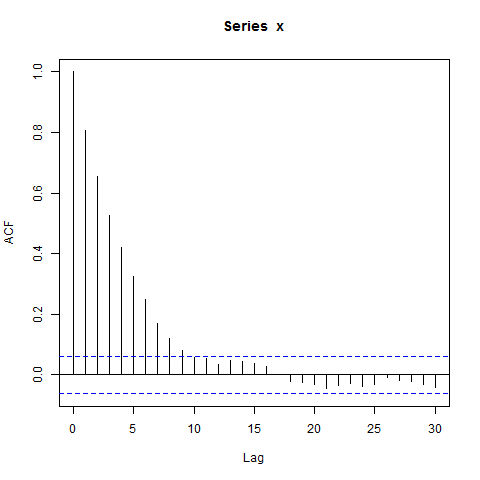
\includegraphics[scale=0.4]{acfnorm.png}

The traceplot suggests that the sampler has traversed through the entire probability. However, the correlation between successive samples seems to be high, as indicated in the autocorrelation function plot for small lag values. This means that although the sampler is able to cover the entire probability space, it does so very slowly since each successive sample is correlated with previous samples. As a result, each update cannot move very far from previous point.

\item Using similar approach as above, the full conditionals are:
\begin{align*}
X,Y|Z &\sim MVN(\Sigma_{(X,Y),Z}\Sigma_Z^{-1}Z,\Sigma_{X,Y}-\Sigma_{(X,Y),Z}\Sigma_Z^{-1}\Sigma_{Z,(X,Y)}) \\
&=MVN(\begin{bmatrix} 0.1 \\ 0.1\end{bmatrix} \cdot 1 \cdot Z, 
\begin{bmatrix} 1 & 0.9 \\ 0.9 & 1 \end{bmatrix}-\begin{bmatrix} 0.1 \\ 0.1 \end{bmatrix} \cdot 1 \cdot \begin{bmatrix} 0.1 & 0.1 \end{bmatrix}) \\
&=MVN(\begin{bmatrix} 0.1Z \\ 0.1Z \end{bmatrix}, \begin{bmatrix} 0.99 & 0.89 \\ 0.89 & 0.99\end{bmatrix}) \\
Z|X,Y &\sim N(0.052632X+0.052632Y, 0.98947)
\end{align*}


Below are the traceplot and autocorrelation function plot for X:

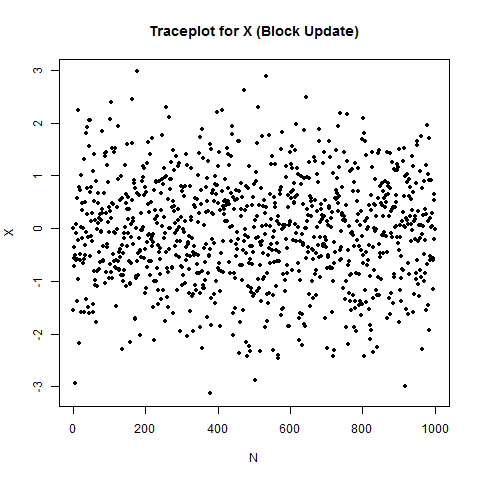
\includegraphics[scale=0.4]{traceblock.png}
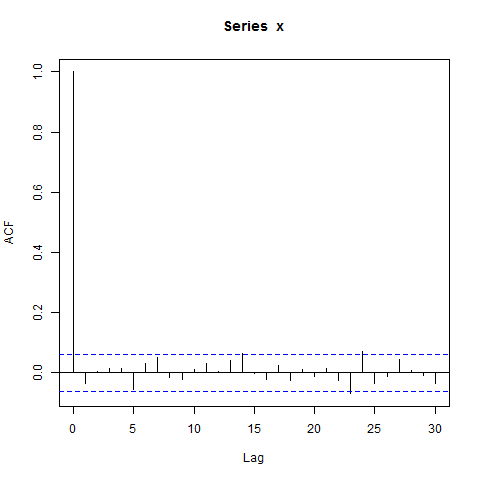
\includegraphics[scale=0.4]{acfblock.png}

The traceplot suggests that this sample has also traversed through the entire probability space. It was able to do so very quickly because successive samples are not highly correlations, as seen in the autocorrelation function plot.

\item Although both samplers seemed to have covered the entire probability space, the normal Gibbs sample was less precise and look longer than block updates because of relatively high autocorrelation. The block updates is more efficient because there was less dependence on conditional variable, i.e., each update requires conditioning twice, whereas the normal Gibbs sampler required conditioning three times.

\end{enumerate}

\pagebreak
R code for normal Gibbs sampler:
\listinginput[1]{1}{gibbs1.r}

R code for block updates:
\listinginput[1]{1}{block.r}


\end{document}